Avec notre billard, est-il possible d'envoyer notre bille pile à l'intersection des deux demi-droites ?
Dans l'exemple ci-dessous, on constate que notre bille s'éloigne sans plus jamais rencontrer de bandes au bout du 5\ieme{} rebond.
 
\medskip

\begin{center}
	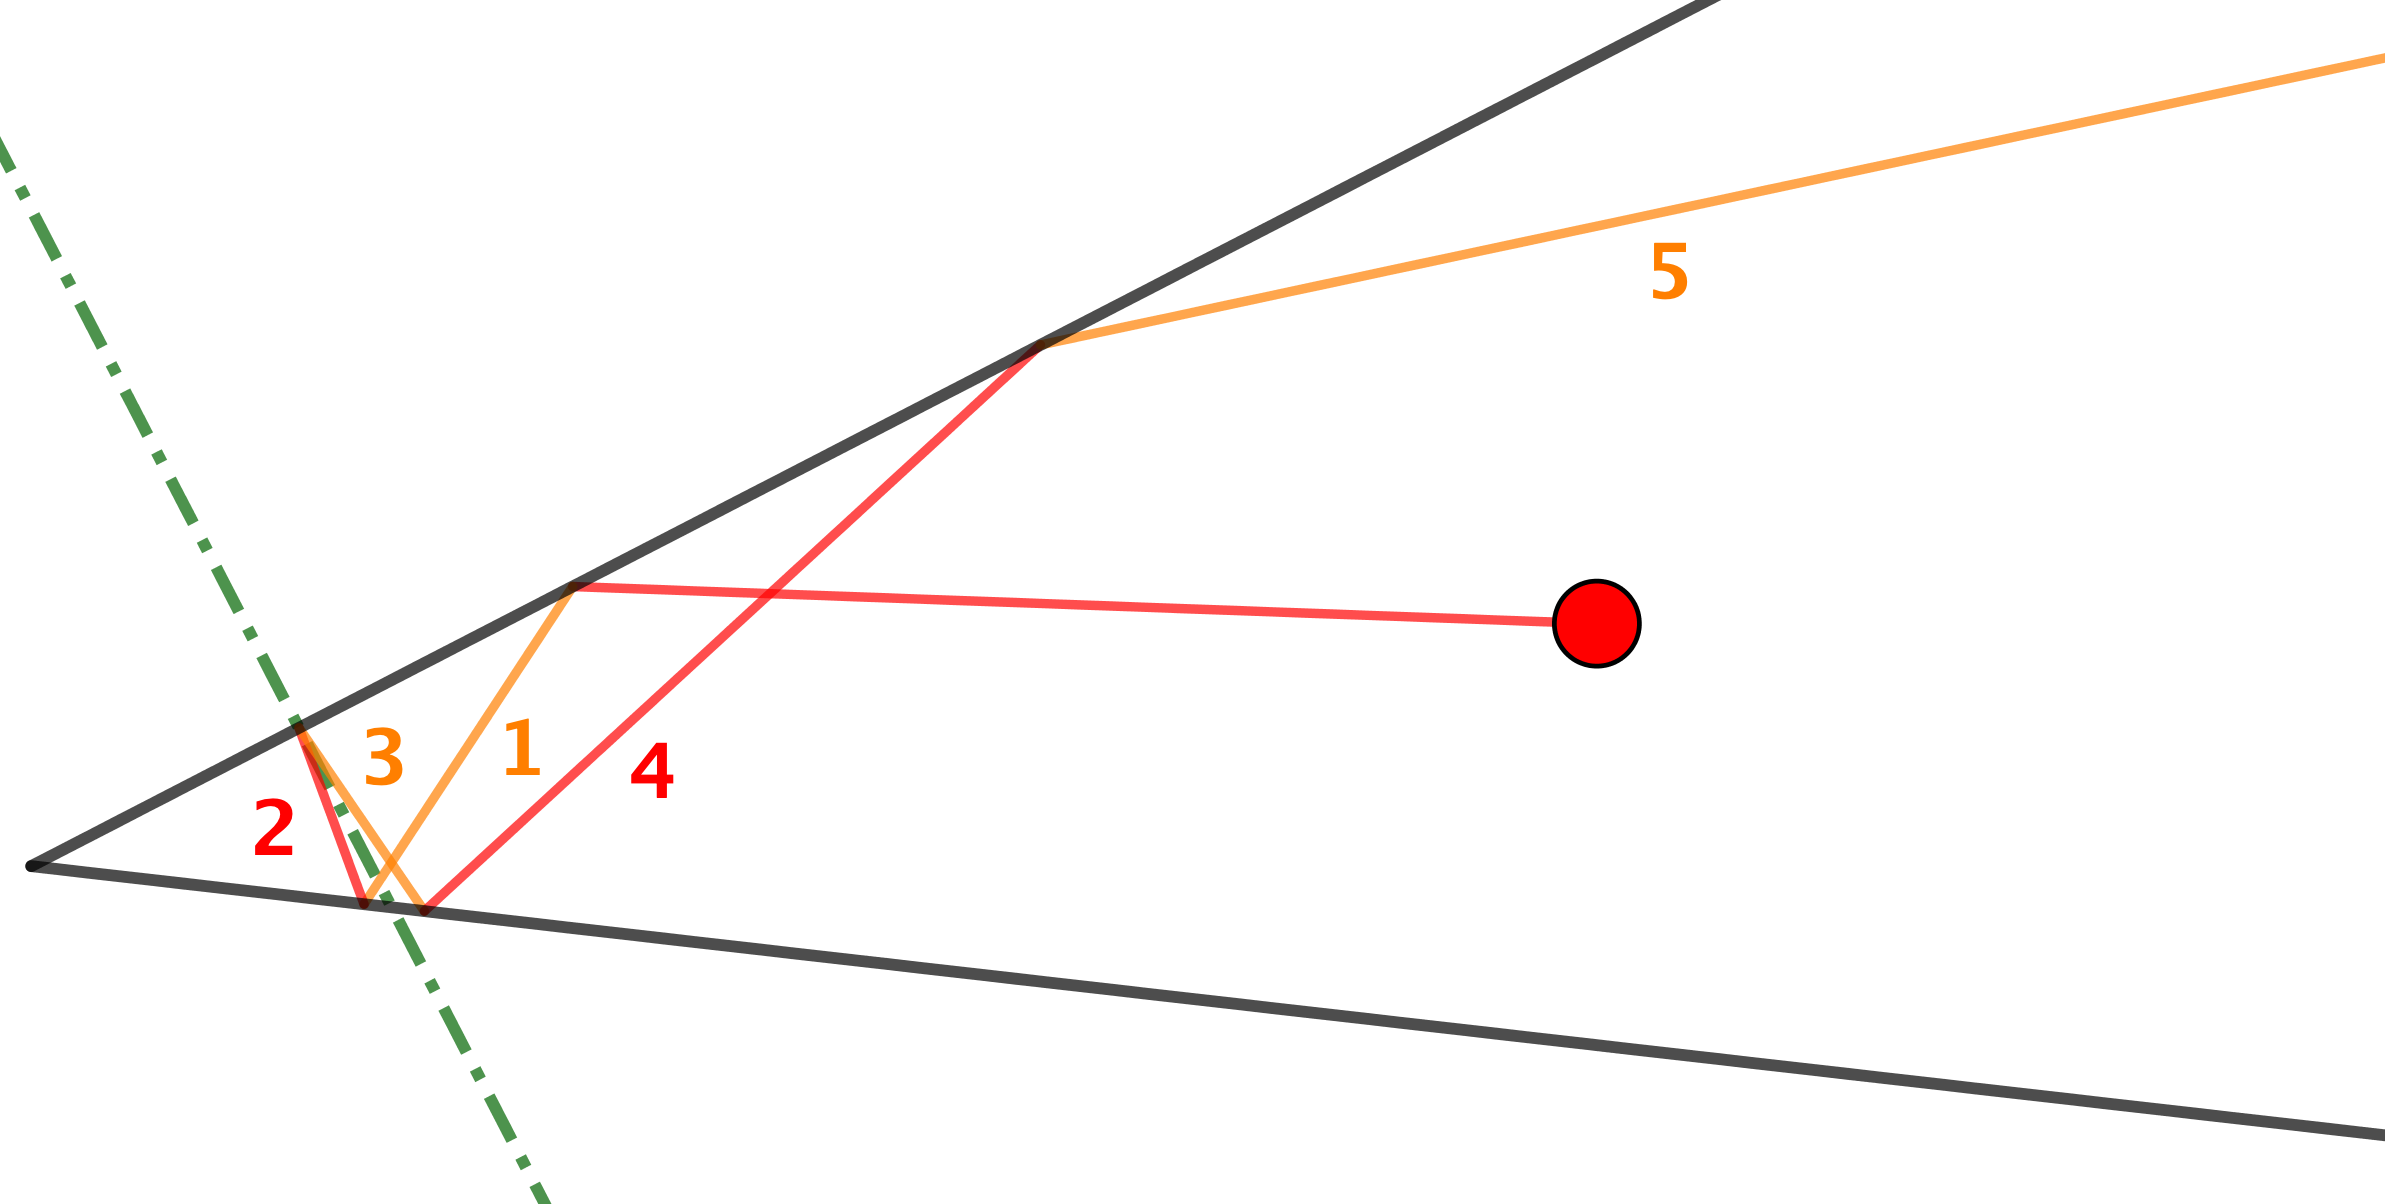
\includegraphics[width=12cm]{content/example-divergence.png}
	
	\itshape\small
	Nous avons laissé une perpendiculaire en pointillés pour les plus sceptiques.
\end{center}

\medskip

En considérant d'autres cas, on se convainc assez vite que la seule façon d'aller au point d'intersection des deux demi-droites, c'est d'y aller directement.
Dès lors que l'on fera une bande, il arrivera toujours un instant où la bille s'éloignera inexorablement. Il reste à démontrer ceci proprement. C'est le but des sections suivantes.